\chapter{Umowy cywilno-prawne}
\label{chap2}
Rozdział ten opisuje umowy cywilno-prawne z prawnego punktu widzenia. Przybliża samo pojęcie umowy oraz prezentuje typy umów, których dotyczy niniejsza praca. Opis ten kładzie szczególny nacisk na ich opodatkowanie i oskładkowanie. Prezentowane są także przykłady osób zatrudnianych na umowy cywilno-prawne. Zawierają one informację o tym, jakie składki powinny być od takich osób odprowadzane. Na koniec dokonany jest krótki przegląd dostępnych na rynku programów wspomagających obsługę umów cywilno-prawnych.

\section[Umowa cywilno-prawna][Umowa cywilno-prawna]{Umowa cywilno-prawna}
Słownik języka polskiego \cite{slownikJP} definiuje umowę jako pisemne lub ustne porozumienie stron, mające na celu ustalenie wzajemnych praw i obowiązków. W polskim prawie jest najważniejszą postacią czynności prawnych. Podstawowe regulacje dotyczące umów zostały umieszczone w części ogólnej Kodeksu cywilnego (art. 66-72) \cite{kodeksCywilny}. Kodeks cywilny reguluje wiele rodzajów umów (m.in. sprzedaży, pożyczki, ubezpieczenia etc...), z których dwie mogą posłużyć jako alternatywne, w stosunku do umowy o pracę, formy zatrudnienia. Są to umowa zlecenia oraz umowa o dzieło.

\subsection[Umowa zlecenia][Umowa zlecenia]{Umowa zlecenia}
Umowa zlecenia została uregulowana przez Kodeks cywilny w art. 734-751 \cite{kodeksCywilny}. Przez umowę zlecenia zleceniobiorca zobowiązuje się do dokonania określonej czynności prawnej dla zleceniodawcy. Umowa zlecenia bywa określana jako umowa starannego działania. Oznacza to, że wynagrodzenie z tytułu umowy zlecenia przysługuje już za samą pracę wykonywaną na rzecz zleceniodawcy, nie zaś za jej rezultat.

\subsection[Umowa o dzieło][Umowa o dzieło]{Umowa o dzieło}
Umowa o dzieło została określona przez Kodeks cywilny w art 627-646\cite{kodeksCywilny}. Najważniejszym jej elementem jest tzw. \textit{Dzieło} - rezultat umowy. Poprzez jej zawarcie sygnatariusze zobowiązują się, z jednej strony do wykonania dzieła, oraz z drugiej strony do wypłaty wynagrodzenia za jego wykonanie. Dziełem może być byt materialny (np. remont budynku), niematerialny (utwór muzyczny, program komputerowy) lub doprowadzenie do ustalonego stanu (np. przeszkolenie pracownika). W momencie zawierania umowy powinno być ono precyzyjnie określone. W przeciwieństwie do umowy zlecenia umowa o dzieło nazywana jest umową rezultatu. Oznacza to, że wynagrodzenie z tytułu umowy o dzieło przysługuje za osiągnięcie konkretnego efektu, a nie za samą pracę (jak w przypadku umowy zlecenia).

\section[Strony umowy][Strony umowy]{Strony umowy}
Wyróżniamy następujące strony stosunku prawnego zaistniałego na podstawie umów cywilno-prawnych:
\begin{itemize}
	\item Zleceniodawcę (dającego zlecenie) - stronę zlecającą wykonanie określonych czynności,
	\item Zleceniobiorcę (przyjmującego zlecenie) - stronę zobowiązującą się do wykonania tych czynności
\end{itemize}
w przypadku umowy zlecenia, oraz
\begin{itemize}
	\item Zamawiającego - stronę zlecającą wykonanie dzieła i zobowiązującą się do wypłaty wynagrodzenia,
	\item Wykonawcę - stronę zobowiązującą się do wykonania dzieła
\end{itemize}
w przypadku umowy o dzieło.

Stronami umowy mogą być zarówno osoby fizyczne jak i osoby prawne.

\section[Forma umowy][Forma umowy]{Forma umowy}
Umowa może zostać zawarta w dowolnej formie, a zatem możemy ograniczyć się do formy ustnej. Zawarcie umowy w formie pisemnej wymaga dla swojej ważności podpisów obu stron. Podpis powinien być podpisem własnoręcznym, dopuszczalny jest też podpis elektroniczny.

\subsection[Elementy obowiązkowe na umowie][Elementy obowiązkowe na umowie]{Elementy obowiązkowe na umowie}
Umowa powinna określać:
\begin{itemize}
\item rodzaj zawartej umowy, która powinna wynikać z nazwy i treści,
\item strony umowy,
\item przedmiot umowy,
\item daty rozpoczęcia i zakończenia wykonywania umowy,
\item informację czy umowa ma być wykonywana u zleceniodawcy bądź zamawiającego,
\item zasady ustalania wynagrodzenia.
\end{itemize}

\section[Wypowiedzenie umowy][Wypowiedzenie umowy]{Wypowiedzenie umowy}
Umowa może być w każdym czasie jednostronnie rozwiązana przez którąkolwiek ze stron. W przypadku umowy odpłatnej zlecający ma obowiązek uiścić wykonawcy bądź zleceniobiorcy część wynagrodzenia odpowiadającą jego dotychczasowym czynnościom. Jeżeli wypowiedzenie nastąpiło bez ważnego powodu, powinien także naprawić wynikłą stąd szkodę. W przypadku gdy umowę wypowiada przyjmujący zlecenie bądź wykonawca dzieła jest on odpowiedzialny za szkodę jaką poniósł zamawiający.

\section[Powierzenie wykonywania umowy osobie trzeciej][Powierzenie wykonywania umowy osobie trzeciej]{Powierzenie wykonywania umowy osobie trzeciej}
Jeśli w umowie nie zostało zapisane, że musi być wykonana osobiście, możliwe jest powierzenie jej wykonania osobie trzeciej.

\section[Wynagrodzenie][Wynagrodzenie]{Wynagrodzenie}
Umowa zlecenia może być zarówno umową odpłatną jak i nieodpłatną, w zależności od ustaleń stron, przy czym jeśli zlecenie ma być nieodpłatne, informacja taka musi znaleźć się w umowie. W przeciwnym razie uznaje się, że zlecenie jest wykonywane odpłatnie. Umowa o dzieło jest zawsze umową odpłatną. Umowa może jednak nie określać dokładnie wysokości wynagrodzenia. Zamiast tego może zawierać podstawy służące do jego ustalenia. Jeśli i tych brak to kwota wynagrodzenia powinna być adekwatna do czasu poświęconego na daną pracę.

Zapłata wynagrodzenia następuje z reguły już po wykonaniu umowy. Strony mogą jednak dowolnie ustalić termin płatności wynagrodzenia, jak i sposób zapłaty (jednorazowy, lub ratalny). Nie ma obowiązku stosowania zasady stosowania comiesięcznej wypłaty przy umowach zawieranych na dłuższy czas. Można pozostać zarówno przy zasadzie rozliczenia po zakończeniu umowy jak i wprowadzić rozliczenia w krótszych okresach.

\section[Rachunek do umowy][Rachunek do umowy]{Rachunek do umowy}
Kwestie rachunków reguluje rozdział 12 Ordynacji podatkowej\cite{ordynacjaPodatkowa}. W ogólnym przypadku nie ma obowiązku wystawiania rachunku do umowy. Obowiązek taki występuję wtedy, gdy zostało to zastrzeżone w umowie lub na życzenie zamawiającego. W takim przypadku rachunek powinien zostać wystawiony w terminie 7 dni od daty wynikającej z umowy lub daty jego zażądania. Rachunek powinien zawierać:
\begin{itemize}
\item numer rachunku - ustawodawca nakłada na wystawiającego obowiązek numerowania rachunków,
\item datę wystawienia,
\item strony umowy,
\item przedmiot umowy,
\item cenę (jednostkową i ogólną - jeśli przedmiot umowy został wykonany kilka razy).
\end{itemize}

\section[Protokół odbioru dzieła lub zlecenia][Protokół odbioru dzieła lub zlecenia]{Protokół odbioru dzieła lub zlecenia}
Podobnie jak w przypadku rachunków Kodeks cywilny nie nakłada obowiązku sporządzania takiego protokołu. Należy go jednak sporządzić jeśli zostało to zaznaczone w umowie. Protokół taki może stanowić podstawę do wypłaty wynagrodzenia bądź wystawienia rachunku. Pozwala też jednoznacznie stwierdzić, że i kiedy nastąpiło odebranie dzieła lub zlecenia.

\section[Opodatkowanie][Opodatkowanie]{Opodatkowanie}
Zasady opodatkowania umów cywilno-prawnych definiuje Ustawa o podatku dochodowym od osób fizycznych\cite{ustawaOPodatkuDochodowym}. W sytuacji, gdy wynagrodzenie z tytułu umowy nie przekracza 200 złotych brutto, przychód podlega opodatkowaniu zryczałtowanym podatkiem dochodowym w wysokości 18\%, bez uwzględniania składek na ZUS i kosztów uzyskania przychodu.
W przypadku wynagrodzenia powyżej 200 złotych brutto, przychód podlega opodatkowaniu na zasadach ogólnych z uwzględnieniem składek ZUS oraz kosztów uzyskania przychodu.

\subsection[Koszty uzyskania przychodu][Koszty uzyskania przychodu]{Koszty uzyskania przychodu}
W myśl art. 22 Ustawy o podatku dochodowym od osób fizycznych\cite{ustawaOPodatkuDochodowym} kosztami uzyskania przychodów są koszty poniesione w celu osiągnięcia przychodów lub zachowania albo zabezpieczenia źródła przychodów. Odlicza się je od wynagrodzenia (po uprzednim odliczeniu składek na ZUS) i dopiero od tak obliczonej kwoty odprowadza się podatek. W większości umów koszty uzyskania przychodu wynoszą 20\% kwoty przychodu netto natomiast w przypadku umów, które wiążą się z przeniesieniem praw autorskich twórców i artystów, koszty uzyskania przychodu wynoszą 50\%. W szczególnych przypadkach koszty te mogą zostać podwyższone, jednak podatnik musi wtedy udowodnić, że poniesione przez niego koszty są faktycznie wyższe niż zapisane w ustawie.

\subsection[Ograniczenia w stosowaniu podwyższonych kosztów uzyskania przychodu][Ograniczenia w stosowaniu podwyższonych kosztów uzyskania przychodu]{Ograniczenia w stosowaniu podwyższonych kosztów uzyskania przychodu}
Od 1 stycznia 2013 roku obowiązuje ograniczenie stosowania 50-procentowych kosztów uzyskania przychodu. Zakłada ono, że  w przypadkach, o których mowa w sekcji \ref{prawaAutorskie}, roczne koszty uzyskania przychodu nie mogą przekroczyć połowy górnej granicy pierwszego przedziału skali podatkowej (1 stycznia 2014 roku wynosiła ona 85 528 zł).

\section[Prawa autorskie][Prawa autorskie]{Prawa autorskie}
\label{prawaAutorskie}
Przypadki, w których możemy korzystać z praw autorskich (a co za tym idzie z podwyższonych kosztów uzyskania przychodu) definiuje art. 22 ust. 9 pkt 1-3 Ustawy o podatku dochodowym od osób fizycznych\cite{ustawaOPodatkuDochodowym}, są to
\begin{itemize}
	\item  zapłata twórcy za przeniesienie prawa własności wynalazku, topografii układu scalonego, wzoru użytkowego, wzoru przemysłowego, znaku towarowego lub wzoru zdobniczego,
	\item opłata licencyjna za przeniesienie prawa stosowania wynalazku, topografii układu scalonego, wzoru użytkowego, wzoru przemysłowego, znaku towarowego lub wzoru zdobniczego, otrzymanej w pierwszym roku trwania licencji od pierwszej jednostki, z którą zawarto umowę licencyjną,
	\item korzystanie przez twórców z praw autorskich i artystów wykonawców z praw pokrewnych, w rozumieniu odrębnych przepisów, lub rozporządzanie przez nich tymi prawami.
\end{itemize}
Typ umowy nie ma w tym przypadku znaczenia. Może to być zarówno umowa zlecenia, umowa o dzieło jak i inna umowa (np. umowa o pracę czy umowa o przeniesienie praw autorskich).

W przypadku omawianych umów cywilno-prawnych umowę o charakterze autorskim należy zawrzeć wtedy, gdy przedmiot umowy stanowi przedmiot prawa autorskiego (utwór) w rozumieniu art. 1 Ustawy o prawie autorskim i prawach pokrewnych\cite{ustawaOPrawieAutorskim}. Przeniesienie praw autorskich wymaga pisemnej formy umowy.

\section[Ubezpieczenia społeczne i ubezpieczenie zdrowotne][Ubezpieczenia społeczne i ubezpieczenie zdrowotne]{Ubezpieczenia społeczne i ubezpieczenie zdrowotne}
Od umów cywilno-prawnych mogą być pobierane składki na następujące ubezpieczenia społeczne:

	\begin{itemize}
		%TODO mozesz dodac opisy poszczególnych ubezpieczeneń
		\item ubezpieczenia emerytalne,
		\item ubezpieczenia rentowe,
		\item ubezpieczenie chorobowe,
		\item bezpiecznie wypadkowe,
	\end{itemize}
oraz ubezpieczenie zdrowotne.

Zasady odprowadzania składek na ubezpieczenia społeczne od umów cywilno-prawnych definiuje rozdział 2 Ustawy o systemie ubezpieczeń społecznych\cite{ustawaOSystemieUbezpieczen} zaś na ubezpieczenie zdrowotne dział IV Ustawy o świadczeniach opieki zdrowotnej finansowanych ze środków publicznych\cite{ustawaOSwiadczeniachOpieki}.

\subsection[Ubezpieczenie emerytalne i ubezpieczenie rentowe][Ubezpieczenie emerytalne i ubezpieczenie rentowe]{Ubezpieczenie emerytalne i ubezpieczenie rentowe}
Obowiązek odprowadzania składek na ubezpieczenia emerytalne i rentowe uzależniony jest od wielu czynników m. in. tego czy osoba zatrudniona na umowę cywilno-prawną ma już podpisaną umowę o pracę, przychodu z tytułu tej umowy czy pracodawcy, z którym umowa została zawarta. Zostanie on wyjaśniony na przykładach w dalszej części rozdziału w sekcji \ref{przykladyOsob}.

\subsection[Ubezpieczenie chorobowe][Ubezpieczenie chorobowe]{Ubezpieczenie chorobowe}
Odprowadzanie składek na ubezpieczenie chorobowe jest możliwe tylko wtedy gdy zatrudniony na umowę cywilno-prawną podlega \textbf{obowiązkowym} ubezpieczeniom emerytalnym i rentowym. W zależności od sytuacji może być ono obowiązkowe lub dobrowolne.

\subsection[Ubezpieczenie wypadkowe][Ubezpieczenie wypadkowe]{Ubezpieczenie wypadkowe}
Zatrudniony na umowę cywilno prawną podlega obowiązkowemu ubezpieczeniu wypadkowemu zawsze wtedy, gdy podlega ubezpieczeniom emerytalnemu i rentowemu (niezależnie od tego czy podlega tym ubezpieczeniom obowiązkowo czy dobrowolnie).

\subsection[Ubezpieczenie zdrowotne][Ubezpieczenie zdrowotne]{Ubezpieczenie zdrowotne}
Zasady odprowadzania składek na ubezpieczenie zdrowotne są zdefiniowane w innej ustawie niż zasady odprowadzania składek na ubezpieczenia społeczne. Dla uproszczenia można przyjąć zasadę, że obowiązek odprowadzania składek na ubezpieczenie zdrowotne ma miejsce wszędzie tam, gdzie występuje obowiązek lub możliwość (ubezpieczenie dobrowolne) odprowadzania składek na ubezpieczenia emerytalne i rentowe. Ustawodawca nie przewidział możliwości dobrowolnego odprowadzania składek na ubezpieczenie zdrowotne.

\section[Przykłady osób zatrudnionych na umowach cywilno-prawnych][Przykłady osób zatrudnionych na umowach cywilno-prawnych]{Przykłady osób zatrudnionych na umowach cywilno-prawnych}
\label{przykladyOsob}

\subsection[Pracownik zatrudniony na umowę o pracę][Pracownik zatrudniony na umowę o pracę]{Pracownik zatrudniony na umowę o pracę}
\label{umowaOPrace}
Jest to przypadek najbardziej złożony. Można go podzielić na 2 mniejsze podprzypadki:

\subsubsection{Umowa cywilno-prawna zawarta z własnym pracodawcą lub wykonywana na rzecz własnego pracodawcy}
W tym przypadku pracodawca ma obowiązek odprowadzać wszystkie ubezpieczenia (emerytalne, rentowe, chorobowe, wypadkowe i zdrowotne) za swojego pracownika.

\subsubsection{Umowa cywilno-prawna nie zawarta z własnym pracodawcą i nie wykonywana na jego rzecz}
W tym przypadku zatrudniony na umowę o dzieło nie podlega (ani dobrowolnie, ani obowiązkowo) żadnemu z ubezpieczeń społecznych ani ubezpieczeniu zdrowotnemu. 

W przypadku umowy zlecenia pod uwagę brany jest przychód z tytułu umowy o pracę. Jeśli jest on niższy od minimalnego wynagrodzenia za pracę (lub jego 80\% w przypadku osób zatrudnionych krócej niż 1 rok) to zleceniobiorca podlega obowiązkowym ubezpieczeniom emerytalnemu, rentowemu i wypadkowemu, może podlegać dobrowolnemu ubezpieczeniu chorobowemu, podlega obowiązkowemu ubezpieczeniu zdrowotnemu. W przeciwnym wypadku może dobrowolnie podlegać ubezpieczeniom emerytalnemu i rentowemu (co pociąga za sobą obowiązkowe podleganie ubezpieczeniu wypadkowemu), nie może podlegać ubezpieczeniu chorobowemu, podlega obowiązkowemu ubezpieczeniu zdrowotnemu. Od 1 stycznia 2014 roku minimalne wynagrodzenie za pracę (tzw. płaca minimalna) wynosi 1680 zł brutto.

\subsection[Uczeń lub student do 26 roku życia][Uczeń lub student do 26 roku życia]{Uczeń lub student do 26 roku życia}
Od umów zawartych ze studentami oraz uczniami szkół ponadgimnazjalnych nie odprowadza się składek na ubezpieczenia społeczne ani na ubezpieczenie zdrowotne. Zwolnienie to rozciąga się na okres do ukończenia przez nich 26 roku życia. Osoby kończące szkołę są traktowanie do 31 sierpnia (do końca wakacji) tak jakby ciągle były uczniami danej szkoły (lub do 30 września w przypadku przyjęcia na studia wyższe). Datą ukończenia studiów jest data złożenia egzaminu dyplomowego. Utrata statusu studenta następuje także w przypadku skreślenia z listy studentów.

\subsection[Osoba niemająca innego tytułu ubezpieczenia niż umowa cywilno-prawna][Osoba niemająca innego tytułu ubezpieczenia niż umowa cywilno-prawna]{Osoba niemająca innego tytułu ubezpieczenia niż umowa cywilno-prawna}
\label{inni}
W tym przypadku występuje obowiązek odprowadzania składek na ubezpieczenia emerytalne, rentowe, wypadkowe oraz ubezpieczenie zdrowotne od umowy zlecenia, oraz możliwość dobrowolnego przystąpienia do ubezpieczenia chorobowego. Jeśli jednak zleceniobiorca podpisze równolegle kilka umów zleceń to znika obowiązek odprowadzania składek na ubezpieczenia emerytalne i rentowe od kolejnych umów (stają się one dobrowolne), nie ma też możliwości podlegania ubezpieczeniu chorobowemu, pozostaje jednak obowiązek podlegania ubezpieczeniu zdrowotnemu (musi być ono odprowadzane od każdej umowy), ubezpieczenie wypadkowe jest uzależnione od ubezpieczeń emerytalnego i chorobowego.

W przypadku umowy o dzieło wykonawca nie podlega ubezpieczeniom społecznym ani ubezpieczeniu zdrowotnemu.

\subsection[Emeryt lub rencista][Emeryt lub rencista]{Emeryt lub rencista}
Emerytów i rencistów obowiązują w ogólności takie same zasady jak osoby niemające innego tytułu ubezpieczenia (patrz \ref{inni}).
Wyjątkiem jest sytuacja, w której emeryt lub rencista jest zatrudniony na umowę o pracę (porównaj \ref{umowaOPrace}). Można tu również wyróżnić 2 przypadki:

\subsubsection{Umowa cywilno-prawna zawarta przez emeryta lub rencistę z własnym pracodawcą lub wykonywana na rzecz własnego pracodawcy}
W tym przypadku pracodawca (tak jak w przypadku zwykłego pracownika) ma obowiązek odprowadzać wszystkie ubezpieczenia (emerytalne, rentowe, chorobowe, wypadkowe i zdrowotne).

\subsubsection{Umowa cywilno-prawna nie zawarta przez emeryta lub rencistę z własnym pracodawcą i nie wykonywana na jego rzecz}
W przypadku umowy o dzieło emeryt lub rencista traktowany jest jak zwykły pracownik i nie podlega ubezpieczeniom społecznym ani ubezpieczeniu zdrowotnemu. Różnica występuje natomiast w przypadku umowy zlecenia. Nie zależnie od przychodu z tytułu umowy o pracę zleceniobiorca jest traktowany tak jakby jego wynagrodzenie ze stosunku pracy było większe bądź równe płacy minimalnej. Może on wtedy podlegać dobrowolnie ubezpieczeniom emerytalnemu i rentowemu (a co za tym idzie również wypadkowemu), nie może podlegać ubezpieczeniu chorobowemu oraz podlega obowiązkowemu ubezpieczeniu zdrowotnemu.

\subsection[Osoba pobierająca zasiłek macierzyński][Osoba pobierająca zasiłek macierzyński]{Osoba pobierająca zasiłek macierzyński}
W przypadku umów zleceń osoba pobierająca zasiłek macierzyński może dobrowolnie podlegać ubezpieczeniom emerytalnemu i rentowemu (co pociąga za sobą obowiązkowe podleganie ubezpieczeniu wypadkowemu), nie może podlegać ubezpieczeniu chorobowemu, podlega obowiązkowemu ubezpieczeniu zdrowotnemu. W przypadku umów o dzieło osoba taka nie podlega ubezpieczeniom społecznym ani ubezpieczeniu zdrowotnemu.

\subsection[Osoba przybywająca na urlopie wychowawczym][Osoba przybywająca na urlopie wychowawczym]{Osoba przybywająca na urlopie wychowawczym}
Osoba przybywająca na urlopie wychowawczym z punku widzenia ubezpieczeń społecznych i ubezpieczenia zdrowotnego traktowana jest tak osoba niemająca innego tytułu ubezpieczenia niż umowa cywilno-prawna (patrz \ref{inni}).

\subsection[Osoba prowadząca działalność gospodarczą][Osoba prowadząca działalność gospodarczą]{Osoba prowadząca działalność gospodarczą}
Jeśli umowa cywilno-prawna jest wykonywana w ramach prowadzonej działalności gospodarczej to nie podlega ona ubezpieczeniom społecznym ani ubezpieczeniu zdrowotnemu. W przeciwnym wypadku osoba zatrudniona na taką umowę powinna być traktowana jak osoba zatrudniona na umowę o pracę u pracodawcy innego niż zleceniodawca bądź zamawiający dzieło (patrz \ref{umowaOPrace}).

\section{Składki na Fundusz Gwarantowanych Świadczeń Pracowniczych i Fundusz Pracy}
Obowiązek odprowadzania składek na Fundusz Gwarantowanych Świadczeń Pracowniczych i Fundusz Pracy regulują odpowiednio: Ustawa o ochronie roszczeń pracowniczych w razie niewypłacalności pracodawcy\cite{ustawaOOchronieRoszczen} i Ustawa o promocji zatrudnienia i instytucjach rynku pracy\cite{ustawaOPromocjiZatrudnienia}. Obowiązek taki występuje gdy zatrudniony na umowę cywilno-prawną:
\begin{itemize}
	\item podlega obowiązkowym ubezpieczeniom emerytalnemu i rentowym oraz
	\item uzyskuje z tytułu umowy przychód w wysokości co najmniej minimalnego wynagrodzenia za prace.
\end{itemize}
Składek na Fundusz Gwarantowanych Świadczeń Pracowniczych i Fundusz Pracy nie odprowadza się po ukończeniu 55 lat (w przypadku kobiet) lub 60 lat (w przypadku mężczyzn).

\section[Umowy cywilno-prawne a prawo pracy][Umowy cywilno-prawne a prawo pracy]{Umowy cywilno-prawne a prawo pracy}
W przypadku umów cywilno-prawnych nie zachodzi stosunek pracy, nie ma więc zastosowania prawo pracy (w szczególności kodeks pracy). Zatrudniony na taką umowę nie ma więc prawa do płatnych urlopów. Nie ma również możliwości korzystania ze zwolnienia lekarskiego.

\section[Systemy wspomagające obsługę umów cywilno-prawnych][Systemy wspomagające obsługę umów cywilno-prawnych]{Systemy wspomagające obsługę umów cywilno-prawnych}

\subsection[Kalkulatory wynagrodzeń][Kalkulatory wynagrodzeń]{Kalkulatory wynagrodzeń}
Do najprostszych przykładów aplikacji wspomagających obsługę umów cywilno-prawnych należą kalkulatory wynagrodzeń. Pozwalają one na obliczanie wynagrodzenia netto na podstawie podanego wynagrodzenia brutto, oraz informacji o koszcie uzyskania przychodu oraz składkach odprowadzanych na ubezpieczenia społeczne i ubezpieczenie zdrowotne. Na rysunku \ref{kalkulator} przedstawiono przykładowy kalkulator dostępny w internecie na stronie www.kalkulatory.gofin.pl.

\begin{figure}[tdh]
    \begin{center}
	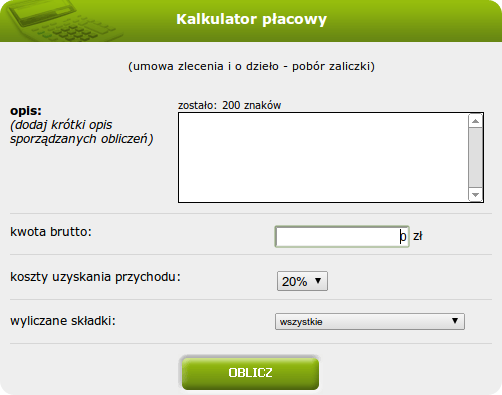
\includegraphics[scale=.6]{img/kalkulator.png}
	\caption{Kalkulator wynagrodzeń z tytułu umów cywilno-prawnych}
	\label{kalkulator}
    \end{center}
\end{figure}

\subsection[SystemUmów.pl][SystemUmów.pl]{SystemUmów.pl}
SystemUmów.pl jest dedykowaną aplikacją internetową firmy KotKla do obsługi umów zleceń oraz umów o dzieło. Zapewnia ona przede wszystkim:
\begin{itemize}
	\item dodawanie oraz archiwizację umów,
	\item szablony umów (bogata baza dostępnych szablonów oraz możliwość definiowania własnych),
	\item dodawanie pracowników oraz przechowywanie ich danych,
	\item ręczne generowanie rachunków na podstawie szablonów (wbudowanych lub zdefiniowanych własnoręcznie),
	\item eksport umów i rachunków do formatu pdf,
	\item miesięcznie oraz roczne deklaracje PIT i ZUS,
	\item możliwość definiowania danych (takich jak nazwa, adres, numery NIP czy REGON) własnej firmy.
\end{itemize}

Jest to aplikacja płatna (150 zł za rok bądź 3000 zł za licencję dożywotnią), ale istnieje też jej darmowa wersja. Charakteryzuje się ona następującymi ograniczeniami:
\begin{itemize}
	\item czas trwania licencji ograniczony do 90 dni,
	\item liczba własnych szablonów ograniczona do 3,
	\item liczba umów ograniczona do 50.
\end{itemize}
Program pozwala na łatwe realizowanie podstawowych funkcji związanych z obsługą umów cywilno-prawnych, łatwo jednak zauważyć kilka podstawowych ograniczeń.
\begin{itemize}
	\item możliwość generowania tylko jednego rachunku do każdej umowy - nie pozwala to na ratalną wypłatę wynagrodzenia.
	\item ręczne generowanie rachunku na podstawie szablonu pozwala wygenerować rachunek nieadekwatny do umowy (np. rachunek informujący o 50\% koszcie uzyskania przychodu do nieautorskiej umowy), wymaga też znajomości składek ZUS pracownika.
	\item brak możliwości podziału przedsiębiorstwa na mniejsze jednostki, czy wyodrębniania poszczególnych zadań.
\end{itemize}

Na rysunku \ref{kotkla-systemumow} przedstawiono przykładowy zrzut ekranu z aplikacji SystemUmów.pl

\begin{figure}[tdh]
    \begin{center}
	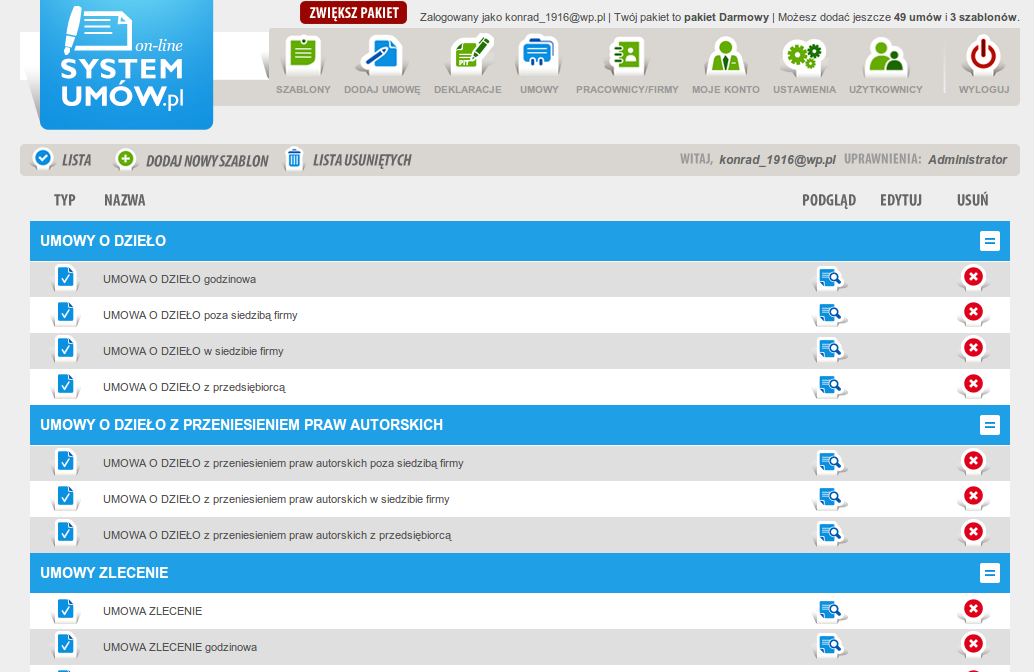
\includegraphics[scale=.4]{img/kotkla-systemumow.png}
	\caption{Lista szablonów umów cywilno-prawnych w aplikacji KotKla-SystemUmów.pl}
	\label{kotkla-systemumow}
    \end{center}
\end{figure}

\subsection[Asystent Rejestr Umów][Asystent Rejestr Umów]{Asystent Rejestr Umów}
Asystent Rejestr Umów to program firmy Meteoryt Software. Ma on postać aplikacji desktopowej korzystającej z bazy danych (lokalnej lub zdalnej). Jest to bardzo zaawansowana aplikacja pozwalająca nie tylko na obsługę umów, ale też na zarządzanie zadaniami, danymi kontraktowymi, wspierająca system sprzedaży czy służąca do fakturowania. Wśród wspieranych przez nią umów są, obok umów zleceń i o dzieło, umowy takie jak umowa o pracę czy umowa kupna-sprzedaży. Zapewnia obsługę takich szczegółów jak okres wypowiedzenia czy miejsce przechowywania oryginału umowy. Pozwala na wysyłanie notyfikacji w formie e-maili bądź smsów. Jest oczywiście aplikacją płatną, a jej ceny wahają się w zależności od wersji (najtańszą wersja PRO kosztuje 99zł za rok użytkowania). Na rysunku \ref{asystent-rejestr-umow} przedstawiono przykładowy zrzut ekranu z aplikacji Asystent Rejestr Umów.

\begin{figure}[tdh]
    \begin{center}
	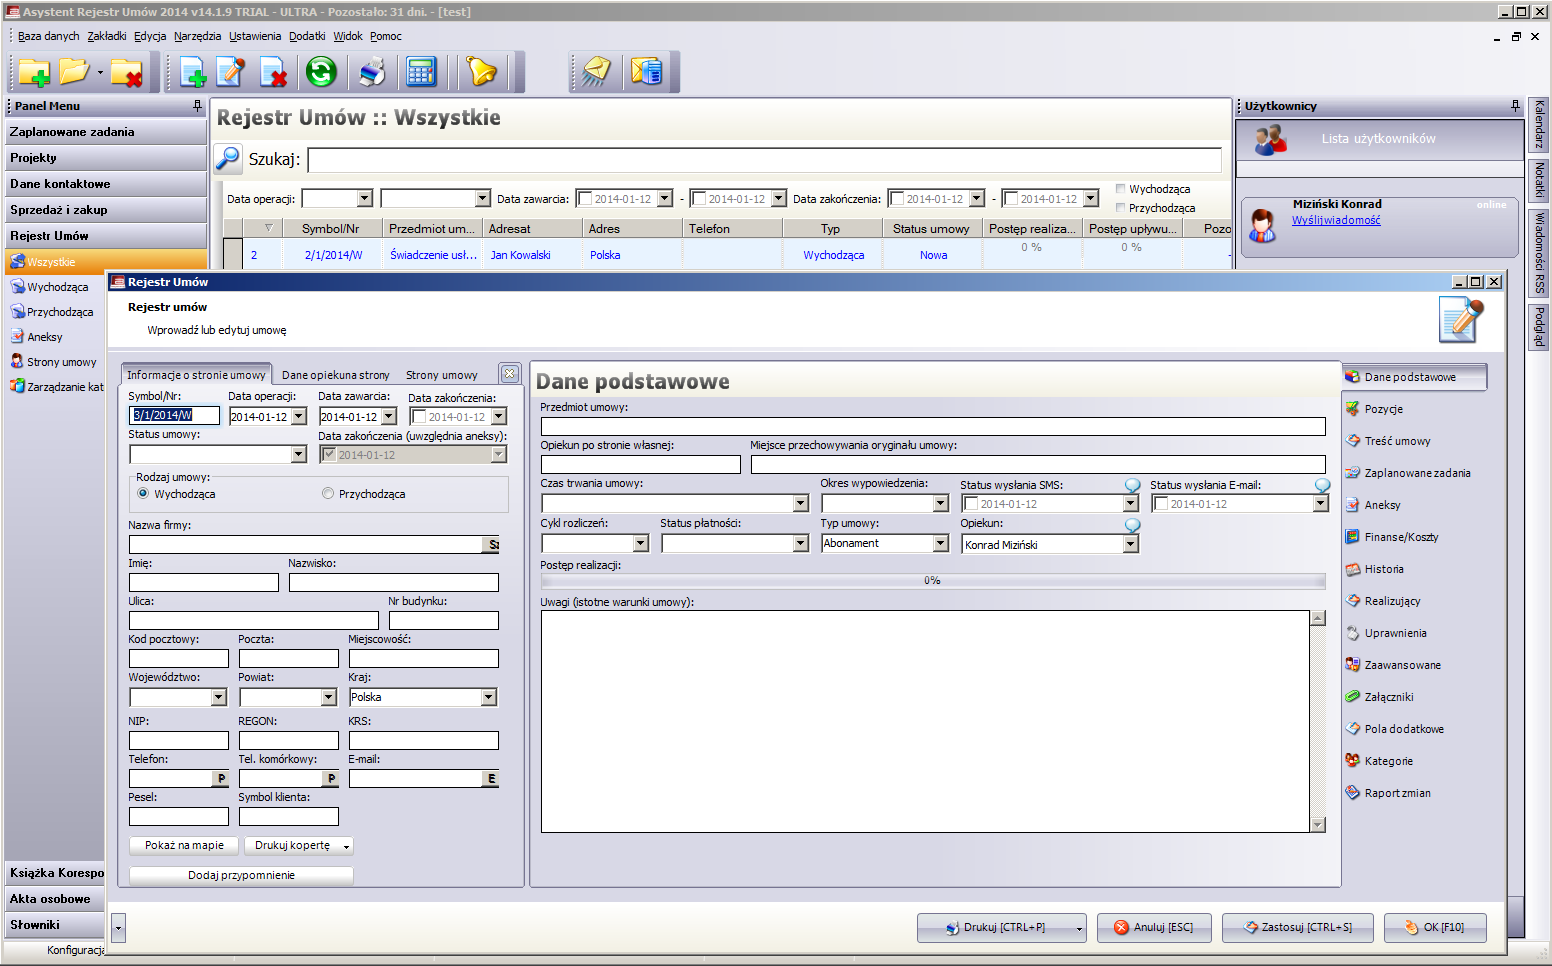
\includegraphics[scale=.6, angle=-90]{img/asystent-rejestr-umow.png}
	\caption{Dodawanie nowej umowy w aplikacji Asystent Rejestr Umów}
	\label{asystent-rejestr-umow}
    \end{center}
\end{figure}
